\documentclass[t]{beamer}
\usepackage[portuguese]{babel}
\usepackage[utf8]{inputenc}
\usetheme{Berkeley}
\usecolortheme{seahorse}

\addto\captionsportuguese{
	\renewcommand{\figurename}{Fig.}
	\renewcommand{\tablename}{Tab.}
}

\title{Micro processadores e controladores}
\subtitle{Suas características principais e sua importância para a área de IoT.}

\AtBeginSection[]
{
	\begin{frame}
	\frametitle{Sumário}
	\tableofcontents[currentsection]
\end{frame}
}

\begin{document}

\frame{\titlepage}

\begin{frame}
\frametitle{Sumário}
\tableofcontents
\end{frame}

\section{Características}

\begin{frame}{O que é um micro-processador?!}
\begin{itemize}
\item Única CPU
\item Interrupções
\item Clock
\item Utiliza-se de recursos externos (memória, I/O)
\end{itemize}
\end{frame}

\begin{frame}{O que é um micro-controlador?!}
\begin{itemize}
\item Computador em um Chip
\item Design embarcado
\item Interrupções
\item Clock
\item Programável
\end{itemize}
\end{frame}

\section{Arquiteturas}

\begin{frame}{Arquiteturas}
\begin{itemize}
\item Von Neumann
\item Harvard
\end{itemize}
\end{frame}

\begin{frame}{Arquiteturas}
Von Neumann

\begin{figure}
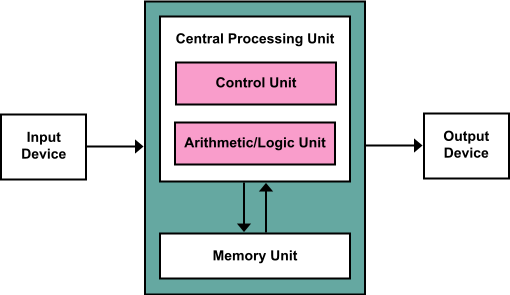
\includegraphics[width=\linewidth]{arquiteturavonneumann}
\end{figure}
\end{frame}

\begin{frame}{Arquiteturas}
Harvard
\begin{figure}
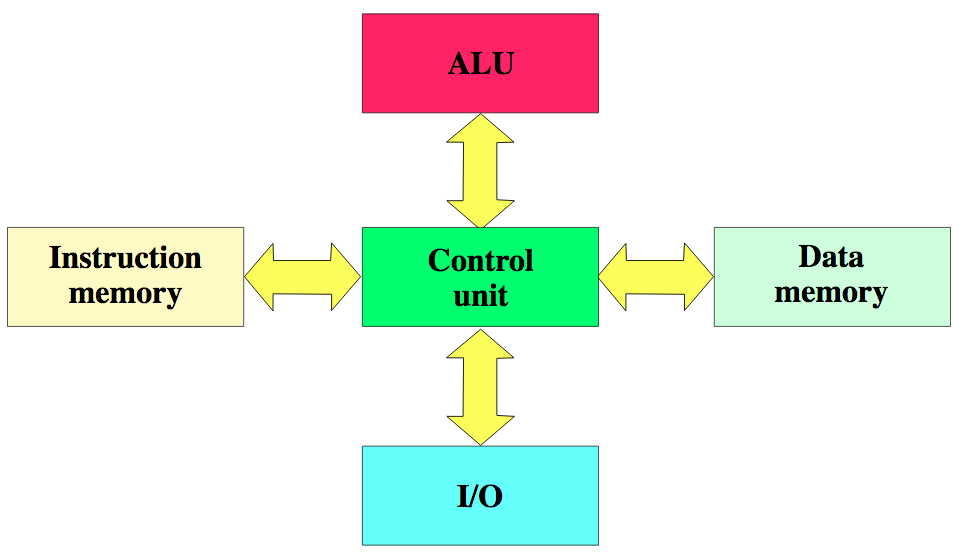
\includegraphics[width=\linewidth]{arquiteturaharvard}
\end{figure}
\end{frame}

\begin{frame}{Arquiteturas}
Comparação
\begin{columns}
\begin{column}{0.5\linewidth}
\begin{figure}
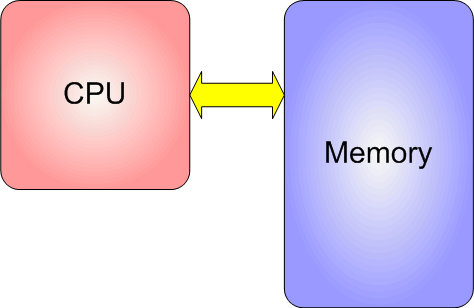
\includegraphics[width=\linewidth]{learn_arduino_Von_Neumann}
\caption{Von Neumann}
\end{figure}
\end{column}
\begin{column}{0.5\linewidth}
\begin{figure}
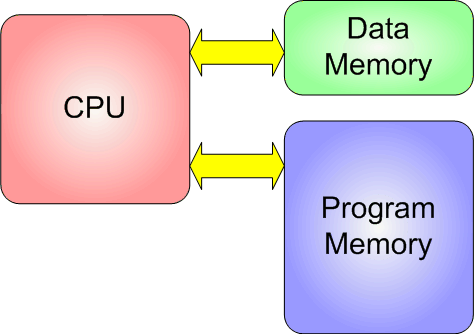
\includegraphics[width=\linewidth]{learn_arduino_Harvard}
\caption{Harvard}
\end{figure}
\end{column}
\end{columns}
\end{frame}

\begin{frame}{Arquiteturas}
Conjuntos de Instruções
\begin{itemize}
\item CISC (Complex Instruction Set Computer)
\item RISC (Reduced Instruction Set Computer)
\end{itemize}
\end{frame}

\section{Processadores}

\begin{frame}{Processadores}
Características
\begin{itemize}
\item Arquiteturas
\item Memórias
\item Clock
\item BUS
\end{itemize}
\end{frame}

\section{Memórias}

\begin{frame}{Memórias}
\begin{itemize}
\item ROM
\item PROM (programmable read-only memory)
\begin{itemize}
\item EPROM
\item EEPROM
\item UV-EPROM
\end{itemize}
\item FLASH
\item RAM
\end{itemize}
\end{frame}

\section{Pinagem}

\begin{frame}{Pinagem}
\begin{itemize}
\item Vin
\item GND
\item RST
\item CLK
\item RX
\item TX
\item GPIO
\item I2C
\end{itemize}
\end{frame}

\section{Exemplos}

\begin{frame}{Exemplos}
Micro-processadores
\begin{itemize}
\item Intel
\begin{itemize}
\item Quark SoC
\end{itemize}
\item Broadcom
\begin{itemize}
\item BCM2835 SoC
\end{itemize}
\item Arm
\begin{itemize}
\item ARM11
\item Cortex A8,A15,A20
\end{itemize}
\end{itemize}
\end{frame}

\begin{frame}{Exemplos}
Micro-controladores
\begin{itemize}
\item Arduino
\item Atmel AVR
\item PIC (Microchip Technology)
\end{itemize}
\end{frame}

\begin{frame}{Exemplos}
Arduino
\begin{figure}
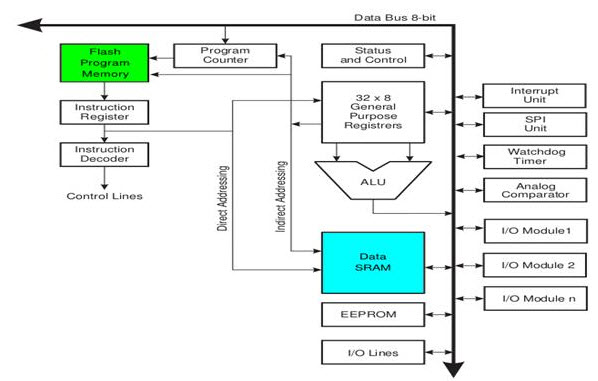
\includegraphics[width=\linewidth]{Arduino-Architecture}
\end{figure}
\end{frame}

\begin{frame}{Exemplos}
ATMega 328 - Diagrama de blocos
\begin{figure}
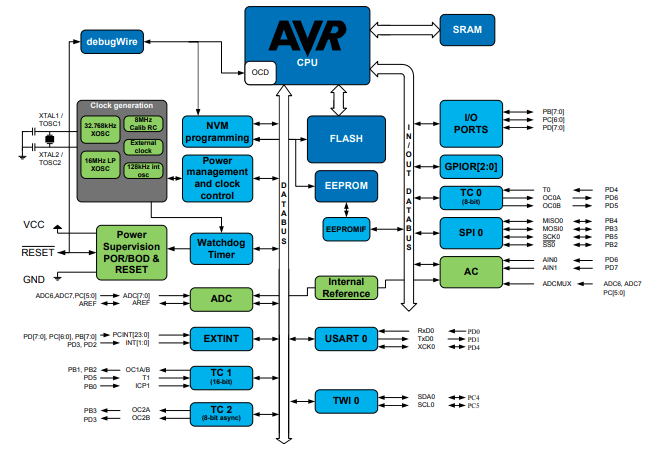
\includegraphics[width=\linewidth]{atmega328-blockdiagram}
\end{figure}
\end{frame}

\begin{frame}{Exemplos}
Placas
\begin{itemize}
\item Raspberry Pi
\item Cubieboard
\item BeagleBone
\item NVidia
\end{itemize}
\end{frame}

\frame{\titlepage}

\end{document}
